%\documentclass{cmspaper}
%\begin{document} 

\section{Data-driven techniques for background estimate} \label{sec:bkgStudy}
After the event selection the dominant number of SM background events in the two electron and two jet sample (eejj sample) 
come from $t\bar{t}$ and $Z/\gamma$+jet processes, as summarized in table \ref{tab:EventSelSummary}. 
This section describes data-driven techniques used to estimate the absolute 
normalization for these two backgrounds, and the shape of selection variable 
distributions for $t\bar{t}$ background using control samples. 
%These shapes are used in a fit to the data to extract the number of signal events, as described 
%in section \ref{sec:signalExtraction}. 
The methods for background estimation described here are based on data and complemented by some Monte Carlo information. 
They are therefore particularly suited for first data taking when confidence that the MC describes
the data well is expected to be limited.

For our analysis, the main properties of a control sample to estimate a background $X$ are:
\begin{itemize}
%
\item to be enriched in $X$ events.
%
\item to be independent from the signal sample;
%
\item to have similar topology of the $X$ events in the signal sample (i.e. eejj sample) 
concerning a given set of reconstructed selection variables under investigation;  
%concerning a given set of reconstructed quantities under investigation;  
%
\end{itemize}
%
The control samples for the $t\bar{t}$ and $Z/\gamma$+jet backgrounds discussed below both satisfy these three conditions.

% NOTE: the more detailed discussion on different amount of background should be discussed in the section Event Selection 
% when you show the table with the number of selected events

%The four main source of background events that pass the High Level Trigger are ttbar, Z+jets, QCD and W+jets.  The application of the electron isolation criteria sufficiently limits the number of fake electrons in the offline selection that the QCD and W+jets background are negligible.  The small contribution of the events with fake electrons from the QCD and W+jet channels can be seen in figure~\ref{fig:Mej_allComb}.

\subsection{$t\bar{t}$ background control sample}

The normalization and the shape of the main selection variable distributions for 
$t\bar{t}$ events can be estimated directly from data using a control sample. 
The basic idea is to select events that are independent from the eejj sample, and have, for the main selection variables, 
shape and resolution similar to the $t\bar{t}$ component in the eejj sample.

A good control sample can be obtained by using the same selection criteria applied for the eejj sample, but 
requiring at least one electron and one muon (e$\mu$jj sample) instead of at least 2 electrons 
in the final state in addition to the two jets. 
For $t\bar{t}$ events, the selection variable distributions of the e$\mu$jj and the eejj samples
are expected to be very similar in shape since the kinematics of the process does not depend 
on the nature of the lepton. Figure~\ref{fig:ttbar} shows a good agreement between 
the shape of $M_{lj}$ and $S_{T}$ distributions with the current MC statistics available. Similar agreement 
is found also for the other reconstructed kinematic variables used in the selection. 

The e$\mu$jj sample is dominated by $t\bar{t}$ events, as shown in Figure~\ref{fig:emujjContamination} 
with a small contamination estimated from MC of less than 5\% (with $S_{T}$ cut of 300 GeV), 
mainly from di-boson events (for $W$+jets and $Z/\gamma$+jets contributions, uncertainties are large, 
around 100\%, due to limited MC statistics). 
The QCD background contamination in the e$\mu$jj sample is not evaluated here, and it's expected to be small. 
The MC statistics of QCD sample is not sufficient to perform a reasonable estimate at this stage, althought 
it seems to confirm the expectation; the plans of using data driven methods to estimate such background will be discussed later in Section XXX. 
For $t\bar{t}$ events the e$\mu$jj sample with 100 pb$^{-1}$ of data 
is expected to have about 66, 11, and 5 events, respectively for an $S_{T}$ cut of 300, 520, and 620 GeV.

For a sample of $t\bar{t}$ events at generator level, the number of e$\mu$jj events is expected to be exactly two times the number of 
eejj events, considering all the possible combinations of the $W$ decays. In general, the trigger filter, the offline selection, 
and the different reconstruction efficiency, acceptance and $P_{T}$ resolution between electron and muon
put a bias in the relative amount of eejj and e$\mu$jj events. 
In this analysis the effect of the different reconstruction efficiency between electrons and muons 
(which is the dominant effect for the current selection) 
is considered, in order to estimate the number of eejj in the signal sample directly from 
the size of the e$\mu$jj control sample. The estimate of the number of events in the eejj sample, 
$N_{eejj}^{est.}$, is extracted from the e$\mu$jj sample accordingly with the relation 

\begin{equation} \label{formula:NeejFromNemujj}
N_{eejj}^{est.} = \frac{1}{2}\sum_{P_{T}^{\mu}} N_{e\mu jj}(P_{T}^{\mu}) \times R(P_{T}^{\mu}) \quad , 
\end{equation}

where $N_{e\mu jj}(P_{T}^{\mu})$ is the $P_{T}$ distribution for e$\mu$jj events of the muon  
with largest transverse momentum, and $R(P_{T})$ is the ratio between electron 
and muon reconstruction efficiencies as a function of lepton $P_{T}$. The ratio $R(P_{T})$ has been obtained 
using a MC FullSim sample of Z+jets events with an equivalent integrated luminosity of about 300 $pb^{-1}$.
The value of $R(P_{T})$ is found to be between 0.85-0.95 for $30 GeV < P_{T} < 500 GeV$.
Once real data becomes available this ratio could be obtained with $tag\&probe$ method using $Z \rightarrow ee$ and 
$Z \rightarrow \mu\mu$ events (see Section \ref{sec:electronEfficiency}).
A closure test of the method is performed using a MC sample of $t\bar{t}$ events. 
Table~\ref{tab:emujjClosureTest} shows the good agreement within statistical uncertainties between 
the $N_{eejj}^{est.}$, calculated from Equation~\ref{formula:NeejFromNemujj}, 
and the prevision from MC, $N_{eejj}$, for samples selected with a loose $S_{T}$ cut of 300 GeV.   

%{\sl Discussion of how clearly this plot shows similar shape and how this will be used}

\begin{figure}[htb]
  \begin{center}
  \begin{tabular}{cc}
  \resizebox{8cm}{!}{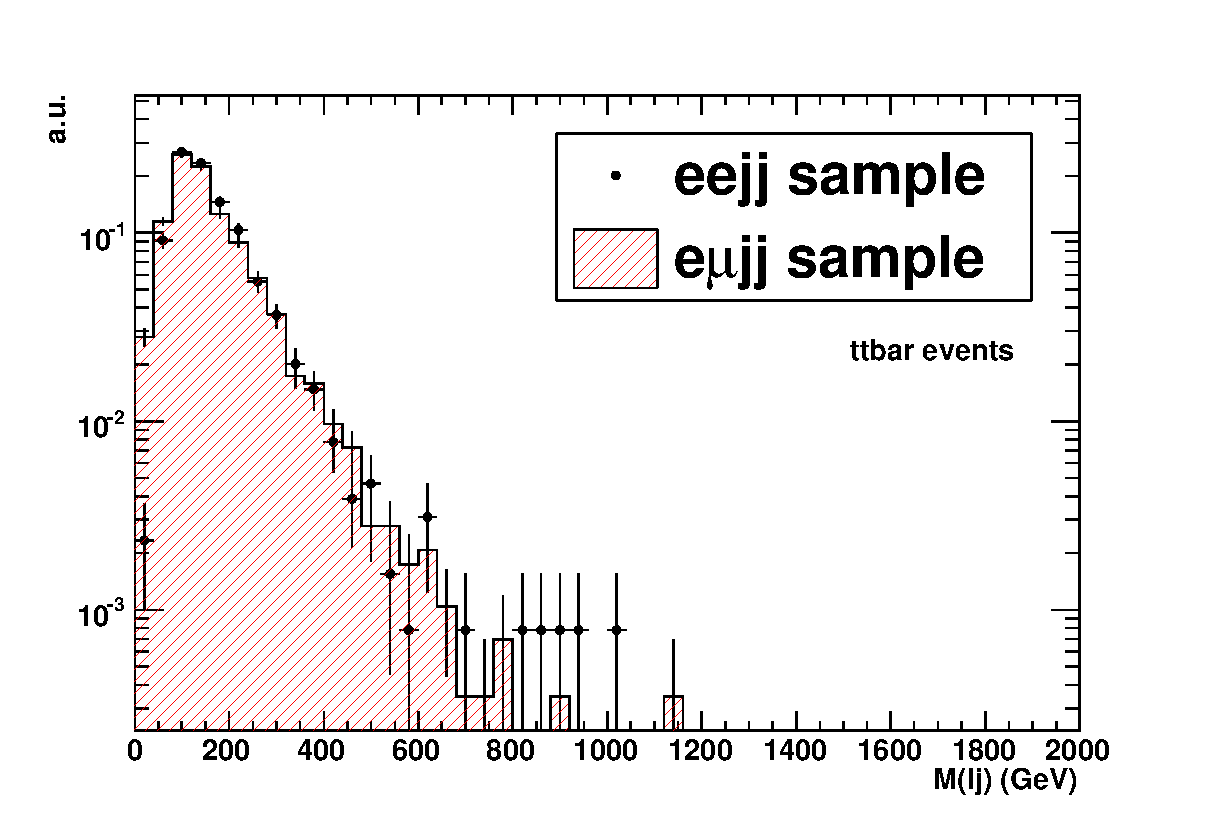
\includegraphics{plots/ttbarStudies/Mlj_eejj_VS_emujj_ttbar_STcut300.eps}} &
  \resizebox{8cm}{!}{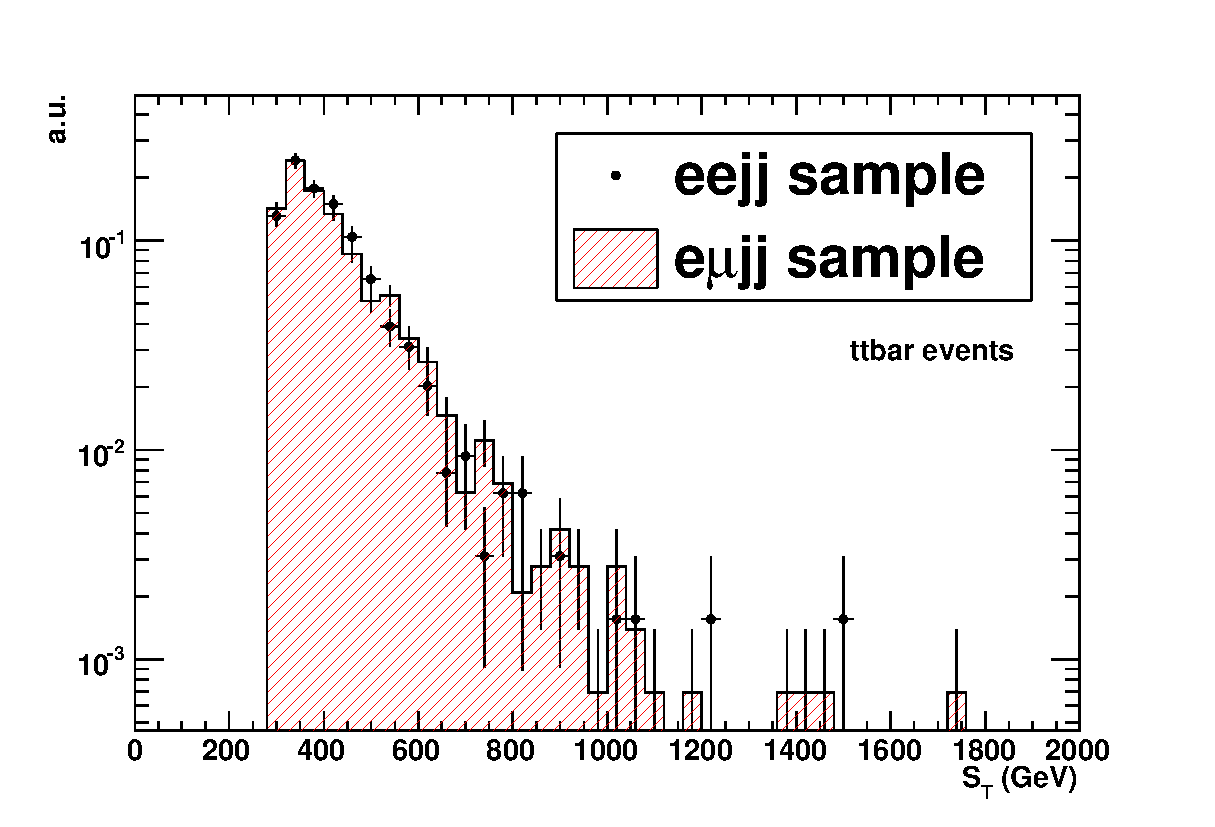
\includegraphics{plots/ttbarStudies/ST_eejj_VS_emujj_ttbar_STcut300.eps}} \\
  \end{tabular}
  \caption{\small \sl Distributions of the lepton-jet invariant mass (left) and $S_{T}$ for the eejj and the e$\mu$ samples, for $t\bar{t}$ events.
  Baseline selection criteria described in Section~\ref{sec:eventSelection} are applied, but the $S_{T}$ cut has been released to 300 GeV.}
  \label{fig:ttbar}
  \end{center}
\end{figure}

\begin{figure}[htb]
  \begin{center}
  \begin{tabular}{cc}
  \resizebox{10cm}{!}{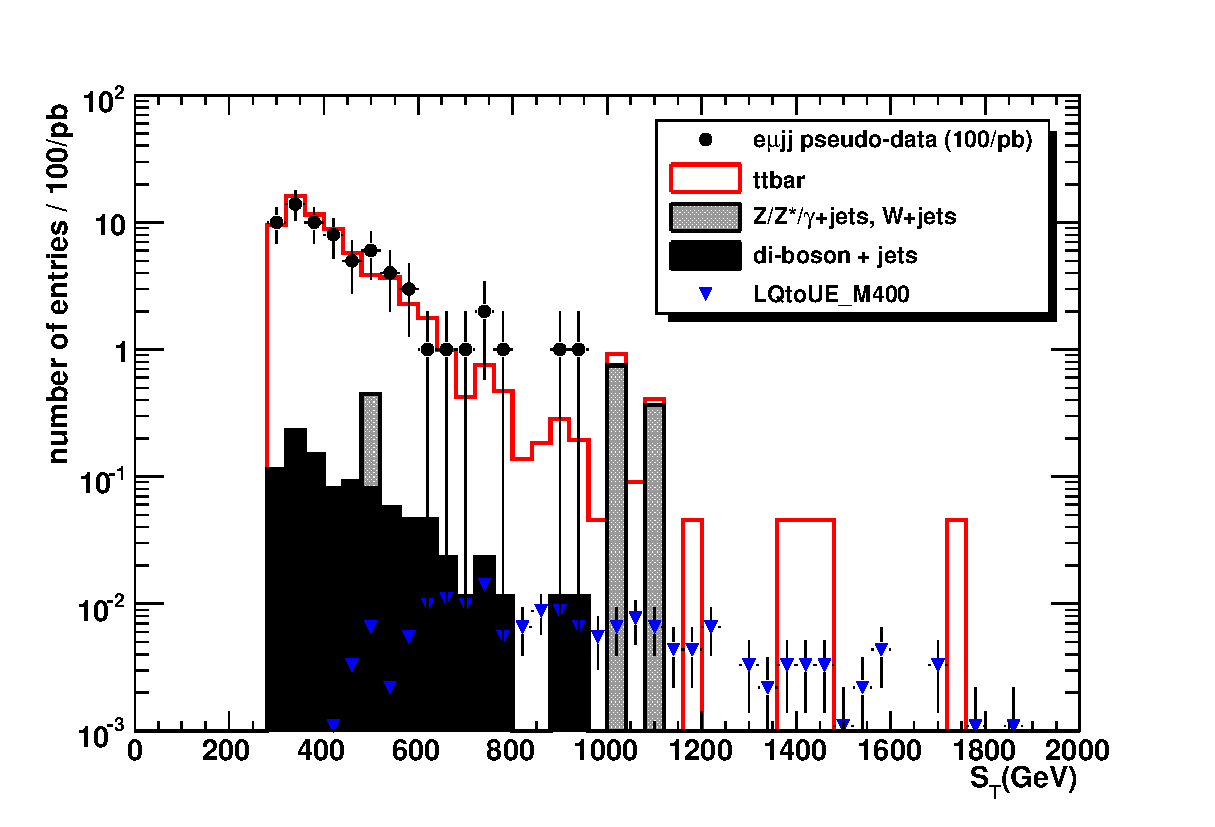
\includegraphics{plots/ttbarStudies/ST_emujj_100pb-1_STcut300.eps}} 
  \end{tabular}
  \caption{\small \sl Distribution of the $S_{T}$ variable for e$\mu$jj sample
    for different background components. 
    Histogram of signal events (at 400~GeV LQ mass) is also added. 
    Baseline selection criteria described in Section~\ref{sec:eventSelection} 
    are applied, but the $S_{T}$ cut has been released to 300 GeV.
    The background histograms are summed on top of each other.
    Black dots indicate pseudo data randomly generated accordingly with 
    the total background distribution, and assuming 100 $pb^{-1}$ of data.}
  \label{fig:emujjContamination}
  \end{center}
\end{figure}


\begin{table}[htb]
  \label{tab:emujjClosureTest}
  \begin{center}
    \begin{tabular}{|l|c|} \hline
      $N_{eejj}$ & 29.4 $\pm$ 1.2 \\ \hline
      $N_{e\mu jj}$ & 65.9 $\pm$ 1.8 \\ \hline \hline
      $N_{eejj}^{est.}$ &  29.5 $\pm$ 0.8 \\ \hline
    \end{tabular}
    \caption{\small \sl $N_{eejj}$ ($N_{e\mu jj}$) is the 
      MC prediction on the number of 
      $t\bar{t}$ events in the eejj 
      (e$\mu$jj) sample with $S_{T}$ cut of 300 GeV, 
      $N_{eejj}^{est.}$ is the number of eejj events estimated
      from the e$\mu$jj sample by using 
      Equation~\ref{formula:NeejFromNemujj}. 
    } 
  \end{center}
\end{table}


\subsection{$Z/\gamma$+jet background control sample} 

A control sample for $Z/\gamma$+jet background estimation (eejjAtZ sample) 
can be obtained by using the same selection criteria applied for the eejj sample except 
the $M_{ee}$ cut, which is modified to select events with a real $Z$ boson reconstructed 
($80\mbox{ GeV} < M_{ee} < 100\mbox{ GeV}$). This control sample is an almost pure sample of  
$Z/\gamma$+jet events as shown in Figure~\ref{fig:eejjAtZContamination}   
( less than 4\% contamination dominated by $t\bar{t}$ events, for $S_{T}$ cut of 300 GeV), 
since the cross section of the process is resonant at the Z mass. 
%the eejjAtZ sample is independent from the eejj signal sample by construction. 
For $Z/\gamma$+jet events, the eejjAtZ sample with 100 pb$^{-1}$ of data 
is expected to have about 129, 22, and 12 events, respectively for an $S_{T}$ cut of 300, 520, and 620 GeV.

The rescaling of the control sample can be obtained with an hybrid method which combines the eejjAtZ data with 
MC information. Once real data is available the eejjAtZ sample can be selected. 
The number of $Z/\gamma$+jet events in the eejj signal sample ($M_{ee}>100$ GeV) can be estimated by

\begin{equation} \label{formula:NeejFromNemujj}
N_{eejj}^{Z} = N_{eejjAtZ} \times R_{OffZ/AtZ} \quad , 
\end{equation}

where $N_{eejjAtZ}$ is the number of events in the eejjAtZ control sample, and 
$R_{OffZ/AtZ}$ is the ratio between the number of $Z/\gamma$+jet events 
with $M_{ee} > 100\mbox{ GeV}$ (OffZ events) and $80\mbox{ GeV} < M_{ee} < 100\mbox{ GeV}$ 
(AtZ events) that have passed all the other selection criteria.
In this analysis the value of $R_{OffZ/AtZ}$ is determined directly from MC.
The motivations that justify this approach are discussed below:
%
\begin{itemize}
%
\item those theoretical uncertainties that are independent 
on the value of two electron invariant mass cancel in the ratio.
In addition, generator level studies will be performed 
in future upgrades of the analysis to quantify the
remaining uncertainties on the value of $R_{OffZ/AtZ}$, 
by using different sets of PDFs and various MC generators.
%
%and eejjAtZ data is used to rescale the $Z/\gamma$ MC sample, 
%thus setting the correct background normalization;
%
\item for inclusive Drell-Yan production ($Z/\gamma \rightarrow ee$ with no jets), 
the MC is expected to predict the value of this ratio with small 
uncertainty (dominated by PDF uncertainties). 
The data-MC comparison will be checked with real data by calculating 
the ratio $R_{OffZ/AtZ}$ using a control sample with only two electrons 
(which is expected to be dominated by Drell-Yan events 
up to values of $M_{ee}$ of several TeV~\ref{HEEPNOTE});%FIXME ADD REFERENCE% 
%
\item the next step will be to compare the distributions of reconstructed selection 
variables between eejjAtZ data and MC to check the agreement in the control region.
It's expected to have more confidence in the MC extrapolation 
from the control region to the signal region (i.e. the estimation of the ratio $R_{OffZ/AtZ}$), 
if the event kinematics in the two regions is not drammatically different.
Figure~\ref{fig:STEleJetceejjAtZvsOffZ}
show the distributions of the scalar sum of $P_{T}$ of the two leading electrons ($S_{T}^{ele}$) 
and the two leading jets ($S_{T}^{jets}$) for $Z/\gamma$+jet events, 
in both signal region (eejj sample) and control region (eejjAtZ control sample). 
A significant discrepancy is observed 
in the $S_{T}^{ele}$ distribution, but this should not represent 
a problem for the MC extrapolation, since the Electro-Weak part of the process 
is well predicted, and this expected agreement could be directly checked with ee data 
(as described in the previous bullet).
It's also comforting that the $S_{T}^{jet}$ distributions are not drammatically different, 
which is an indication that the hadronic part of the $Z/\gamma$+jet process 
(the one with largest uncertainties) is similar between 
signal and control region.  
%
\end{itemize}

%Figure~\ref{fig:zjet} shows the good agreement between eejjAtZ and eejj samples for both the shapes of $M_{ej}$ 
%and $S_{T}$ distributions, using a large FastSim MC sample of $Z/\gamma$+jet events. 
%The agreement observed can be interpreted as the consequence of the 
%weak correlation between the two reconstructed quantities $M_{ej}$ ($S_{T}$) and $M_{ee}$ for selected events, as shown in 
%Figure~\ref{MejVsMeeCorrelation} (Figure~\ref{STVsMeeCorrelation}).

\begin{figure}[htb]
  \begin{center}
  \begin{tabular}{cc}
  \resizebox{10cm}{!}{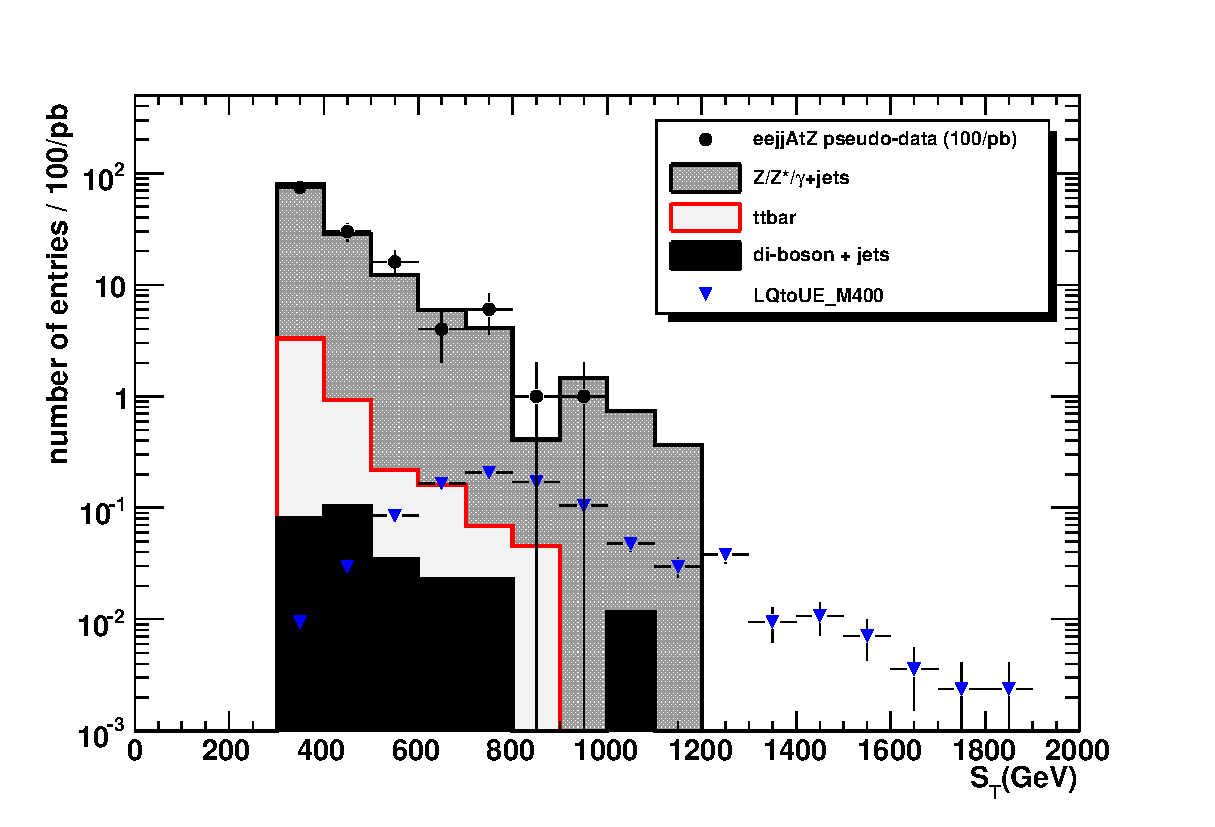
\includegraphics{plots/ZjetStudies/ST_100InVpb_eejjAtZ_looseSTcut_MeeInverted_WithLQ400.eps}} \\ 
  \end{tabular}
%  \caption{\small \sl Distribution of the $P_{T}$ at generator level of the electron pair ($P_{T}$ of the boson) 
%    for $Z/\gamma$+jet events in the signal eejj sample 
%    (cut 1,2,3,4)
%    and the control sample (cut 1,2,4 + $80\mbox{ GeV} < M_{ee} < 100\mbox{ GeV}$), for $Z/\gamma$+jet events.}
  \caption{\small \sl Distribution of the $S_{T}$ variable for eejjAtZ sample
    for different background components. 
    Histogram of signal events (at 400~GeV LQ mass) is also added. 
    Baseline selection criteria described in Section~\ref{sec:eventSelection} 
    are applied, $S_{T}$ cut has been released to 300 GeV, 
    inverted cut on $M_{ee}$ is applied ($80\mbox{ GeV} < M_{ee} < 100\mbox{ GeV}$).
    The background histograms are summed on top of each other.
    Black dots indicate pseudo data randomly generated accordingly with 
    the total background distribution, and assuming 100 $pb^{-1}$ of data.}
  \label{fig:eejjAtZContamination}
  \end{center}
\end{figure}
%
\begin{figure}[htb]
  \begin{center}
  \begin{tabular}{cc}
    a.
    \resizebox{8cm}{!}{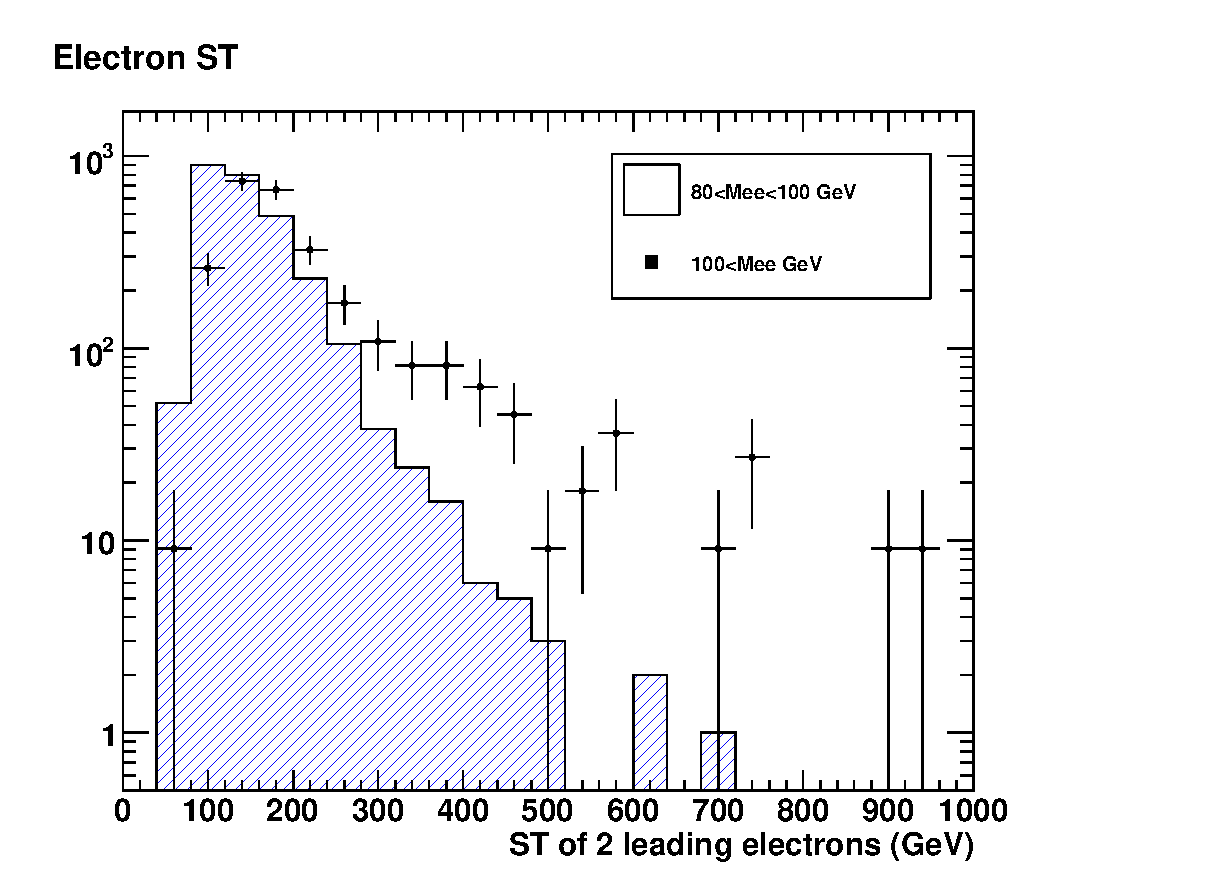
\includegraphics{plots/ZjetStudies/ST_Elecs_inside.eps}} &
    b.
    \resizebox{8cm}{!}{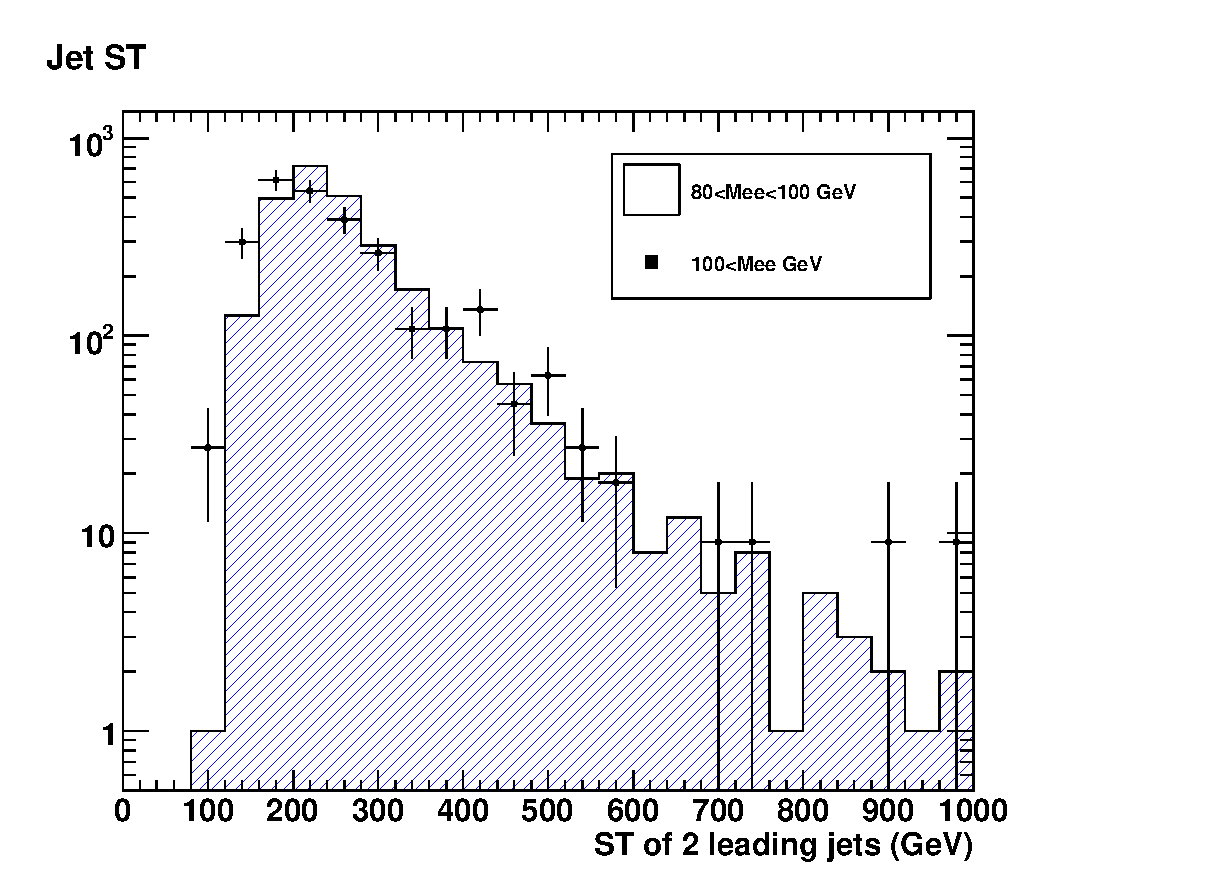
\includegraphics{plots/ZjetStudies/ST_Jets_inside.eps}} \\
  \end{tabular}
  \caption{\small \sl Distributions of (a) $S_{T}^{ele}$ (b) $S_{T}^{jet}$ 
    for the signal eejj sample ($M_{ee} > 100\mbox{ GeV}$) 
    and the eejjAtZ control sample ($80\mbox{ GeV} < M_{ee} < 100\mbox{ GeV}$), 
    using a large FastSim sample of $Z/\gamma$+jet events.}
  \label{fig:STEleJetceejjAtZvsOffZ}
  \end{center}
\end{figure}

%\begin{figure}
%  \begin{center}
%  \begin{tabular}{cc}
%  \resizebox{10cm}{!}{
\includegraphics{plots/UMD.eps}} \\ 
%  \end{tabular}
%  \caption{\small \sl Distribution of the $P_{T}$ at generator level of the electron pair ($P_{T}$ of the boson) 
%    for $Z/\gamma$+jet events in the signal eejj sample 
%    (cut 1,2,3,4)
%    and the control sample (cut 1,2,4 + $80\mbox{ GeV} < M_{ee} < 100\mbox{ GeV}$), for $Z/\gamma$+jet events.}
%  \label{fig:pTeePair}
%  \end{center}
%\end{figure}


%http://cmssw.cvs.cern.ch/cgi-bin/cmssw.cgi/CMSSW/Configuration/CSA07Production/data/CSA07_zjet_ptjgt20_Rmatch0.7_excl.cfg?revision=1.2&view=markup

%alpgen
%zjet_0ptz100gen
%z2j_0ptz100
%njets 2
%ebeam 7000
%ih2 1  - for proton/proton collisions
%ickkw 1 - CKKW prescription for the running of alphas's in the extra gluon emission processes	
%iqopt 1 - renormalization scale
%ptjmin 20
%etajmax 5
%drjmin 0.7
%izdecmode 4

%Fit method (histogram, unbinned, function, combination...)








\subsection{QCD Background} \label{sec:QCDBackground}

FIXME - to be included.




%\end{document}
